\documentclass[../../main.tex]{subfiles}

\subsection{Preámbulo}
\vspace{2mm}
\noindent
En este proyecto se pretende realizar una herramienta en forma de aplicación móvil de
comunicación entre personas, en el que se incluirá como principal componente el
geoposicionamiento de sus usuarios en todo momento. Todo ello, como justificación para el
desarrollo de una infraestructura en el que se aplican novedosos avances actuales en áreas
relacionadas con las arquitecturas de sistemas, orquestación de servicios, seguridad de
servicios web, aplicaciones híbridas móviles, etc.

En el mismo, vamos a intentar desarrollar primero una capa de servicios en la que primen la
seguridad, la alta disponibilidad y la posible tolerancia a fallos. Debido a ello, hemos
decidido aproximarnos a la solución desarrollando una arquitectura de microservicios, los
cuales serán pequeñas piezas funcionales lo mas independientes entre si, en forma de
servicios RESTful, que contarán con distintas infraestructuras de datos dependiendo de los
datos que manejen. Por ejemplo, el servicio que se encarga de posicionar puntos de
encuentro entre usuarios contará con una base de datos \textit{Neo4j} con extensiones espaciales
para controlar la persistencia e indexado de los mismos.

A su vez, para garantizar la disponibilidad de cada uno de los microservicios, aplicaremos
una serie de patrones de sistemas, ampliamente probados a explicar en el memoria, contando para ello
con la ayuda de algunos paquetes de Netflix OSS. La infraestructura se desplegará mediante sistemas de
contenedores (\textit{Dockers}), lo cual nos permite de manera muy rápida realizar réplicas de la
misma ejecutando simplemente un script de código, e incluso levantar réplicas
individuales de cada uno de los microservicios para garantizar una mayor disponibilidad.

Para probar esa infraestructura y mostrar su potencia, vamos a realizar el desarrollo de una
aplicación móvil híbrida mediante el framework de Ionic, que nos ayudará a desarrollarla para
que se pueda desplegar en casi cualquier plataforma con solo una única implementación (code once deploy
everywhere), estando esta diseñada con una aproximación \textit{mobile first}, aunque no se descar\-te
el despliegue en plataformas de corte no móvil.\\

\subsection{Motivaciones}
\vspace{2mm}
\noindent
El proyecto nace en primer lugar como una manera de mostrar los conocimientos adquiridos a lo largo de la consecución del máster, sin olvidar
la idea de mostrar mi capacidad como ingeniero informático para resolver problemas. En él, intento mostrar mis conocimientos del mayor número
posible de tecnologías, así como metodologías, para hacer una puesta en valor de mis capacidades cara al ámbito de la empresa privada.

En segundo lugar, con este proyecto busco abarcar una pequeña iniciación a la temática de una posible línea de investigación de doctorado, en este caso
una iniciación a los datos espaciales, básicamente responder a qué son, cómo se guardan y algunas consultas básicas en los mismos. Para ello, en
este punto de introducción, vamos a dedicar una sección a hablar de los mismos.\\

\subsection{Objetivos}
\vspace{2mm}
\noindent
Teniendo en cuenta las motivaciones de las que nace este trabajo de fin de Master, los objetivos
marcados comprenden una serie de puntos detallados a continuación:
\begin{enumerate}[label=\alph*)]
    \item Realizar un estudio del estado del arte tanto en temas de datos espaciales como en
    desarrollo de arquitecturas de microservicios que me permita una aproximación al
    problema de manera adecuada.
    \item Aprendizaje de las tecnologías pertinentes a la consecución de los objetivos del proyecto. Como por
    ejemplo, Dockers, Ionic, Angular 4, Websockets, Spatial Neo4j, etc.
    \item Enfrentarme a las problemáticas intrínsecas a las arquitecturas devenidas de
    sistemas de alta disponibilidad. Por ejemplo, temas relacionados con la seguridad de la
    infraestructura, tolerancia a fallos de la misma, posibilidad de levantar replicas de los
    servicios de manera rápida y visionado de la misma.
    \item Desarrollo de Whaya (Where Are YA?), una aplicación móvil híbrida que cuente entre
    su funcionalidad como mínimo con un sistema de geoposicionamiento propio y para terceros, así como un chat y la posibilidad de generar encuentros entre usuarios
    amigos.
    \item Elaboración de un artículo valido concluyendo así memoria del proyecto de trabajo
    de fin de máster.
\end{enumerate}

\subsection{Cronograma}
\vspace{2mm}
\noindent
Para cumplir los objetivos descritos anteriormente vamos a mostrar las tareas que nos marcamos en la consecución del proyecto, así como un
diagrama de Gantt para mostrar la temporización de las mismas. Comenzando por las tareas, son las que se muestran a continuación:

\begin{enumerate}[label=\alph*)]
    \item Estudio del problema y análisis. Primero delimitamos lo que queríamos mostrar con la solución dada, así como las tareas preliminares a realizar para la consecución del mismo. 
    \item Estudio de arquitecturas de microservicios y diseño de la arquitectura. Estudiamos el punto en el que están las arquitecturas de microservicios, qué
    decisiones tomar referentes a cómo iban a ser orquestados estos microservicios, y qué tecnologías usaríamos al implementarlos. Junto con ello, tomamos decisiones referentes al diseño de nuestra arquitectura de microservicios.
    \item Aprendizaje de las tecnologías implementadas en el \textit{back-end}. Spring, Netflix OSS, Socket.io, Docker, etc.
    \item Estudio de tecnologías utilizadas en \textit{front-end} y diseño de la aplicación. En este punto tomamos la decision de qué framework utilizar en el \textit{front-end}, cuál sería el diseño de la misma, así como la manera más adecuada de establecer la comunicación con nuestro \textit{back-end}.
    \item Aprendizaje de tecnologías utilizadas en el \textit{front-end}. Ionic, Angular 4, etc.
    \item Implementación del \textit{back-end}.
    \item Implementación del \textit{front-end}.
    \item Depuración, juegos de prueba y corrección de errores.
    \item Preparación de la memoria y presentación. 
\end{enumerate}

Para tener una visión aproximada de lo que ha supuesto la consecución del proyecto (Figura \ref{fig:cronograma}) veamos un diagrama de Gantt aproximado del mismo.

\begin{figure}[H]
    \begin{ganttchart}[vgrid={draw=none,draw=none},%
        %today=15,%
        %today offset=.5,%
        %today label=Heute,%
        %progress=today,%
        x unit=0.3cm,
        y unit title=0.7cm,
        y unit chart=0.5cm,
        bar incomplete/.append style={fill=red},%
        progress label text=  {\quad\pgfmathprintnumber[precision=0,verbatim]{#1}\%},
        milestone label font=\tiny,
        title label font=\tiny,
        bar label node/.style={font=\tiny ,align=right,anchor=east},
        milestone label node/.style={align=right,anchor=east},
        group label node/.style={font=\tiny,align=right,anchor=east}
        ]{1}{36}
        \gantttitle{07/2017 - 12/2017}{24}
        \gantttitle{01/2018 - 03/2018}{12} \\
        \gantttitlelist{07,...,12}{4}
        \gantttitlelist{1,...,3}{4} \\
        \gantttitlelist{1,...,36}{1} \\
        \ganttgroup{Análisis \\ Diseño}{1}{12} \\
        \ganttbar[name=1]{1}{1}{8} \\
        \ganttbar[name=2]{2}{1}{12} \\
        \ganttbar[name=3]{3}{1}{12} \\
        \ganttbar[name=4]{4}{5}{16} \\
        \ganttbar[name=5]{5}{5}{16} \\
        \ganttgroup{Implementación}{13}{26} \\
        \ganttbar[name=6]{6}{17}{24} \\
        \ganttbar[name=7]{7}{20}{26} \\
        \ganttgroup{Pruebas}{27}{29} \\
        \ganttbar[name=8]{8}{27}{29} \\
        \ganttgroup{Documentación}{30}{36} \\
        \ganttbar[name=9]{9}{30}{36} \\
        \ganttlink{2}{6}
        \ganttlink{3}{6}
        \ganttlink{4}{7}
        \ganttlink{5}{7}
        \ganttlink{6}{8}
        \ganttlink{7}{8}
        \ganttlink{8}{9}
    \end{ganttchart}
    \caption{Cronograma del trabajo de fin de master.}
    \label{fig:cronograma}
\end{figure}

\subsection{Datos espaciales}
\vspace{2mm}
\noindent
Los datos espaciales son aquellos que representan la localización, el tamaño o la forma de un objeto partiendo de un sistema de referencia geográfica.
Estos datos también pueden incluir atributos sobre el objeto real que pretende ser representado. Para acceder, visualizar o manipular este tipo de datos, se suelen utilizar
frameworks o herramientas de soporte de Sistemas de Información Geográfica (GIS).

En este proyecto vamos a centrarnos en dos de los frameworks de sistemas \textit{GIS} más utilizados. Por un lado \textbf{PostGIS}, que es una extensión del sistema de base de datos \textit{PostgreSQL}
que la convierte en una base de datos espacial, cuenta con las características descritas en la especificación \textit{OpenGIS} del Open Geospatial Consortium \cite{ogc}. Este sistema es utilizado por infinidad de organizaciones a nivel mundial, su primera versión estable 1.0 data del año 2005. Las
características principales de la misma son:
\begin{enumerate}[label=\alph*)]
\item Incluye tipos geométricos para \texttt{Points}, \texttt{LineStrings}, \texttt{Polygons}, \texttt{Mul\-ti\-Points}, \texttt{MultiLineStrings}, \texttt{MultiPolygons} y \texttt{Geometry Col\-lections}.
\item Predicados espaciales que ayudan a determinar la interacción de geometrías.
\item Operadores espaciales para determinar medidas de este tipo de datos, como pueden ser medidas de área, distancia, etc. A su vez también operaciones entre los datos como pueden ser unión, diferencia, etc.
\item De base trabajan con un \textbf{R-tree-over-GiST} (Generalized Search Tree) para las consultas que requieran de estos índices espaciales.
\item Soporte para la mezcla de índices espaciales y no espaciales mediante planes de consulta.
\item Para datos de rasterización cuentan con \textit{PostGIS Raster}.
\end{enumerate}
\noindent
La ventaja de \textit{PostGIS} es que al ser una implementación basada en \textit{geometrías ligeras} e índices simples, está optimizada para tener un uso de memoria y disco mínimo, lo cual hace que
la cantidad de datos que caben en la RAM sea sustancialmente mayor que en otros sistemas GIS lo que provoca que se mejore la velocidad de las consultas.

Por otro lado también vamos a hablar de \textit{Neo4j Spatial} que es también una extensión en este caso de una base de datos \textit{Neo4j}. Al contrario de \textit{PostgreSQL}, que es una base de datos relacional,
\textit{Neo4j} es una base de datos de las comúnmente llamadas NoSQL, más concretamente una base de datos orientada a grafos, en la que se guardan varios tipos de objetos como entidades (nodos) y sus relaciones (aristas). Para situaciones en las que los datos
se ajustan a este modelo, hacen que esta solución pueda ser mucho más rápidas que otras. Un ejemplo de datos que se ajustan al modelo serian los que nosotros estamos tratando, ya que por ejemplo, podemos considerar algunos nodos como los lugares, y las relaciones como
la rutas de unión de esos lugares.

La mayoría de bases de datos NoSQL se diseñan teniendo en cuenta que deben de cumplirse al menos 2 de las características que son intrínsecas al teorema de CAP, que son:
\begin{enumerate}[label=\alph*)]
\item \textbf{Consistency}. Que viene a significar que las transacciones son ACID, lo cual nos permite confirmar que todos los objetos tienen los mismos datos al mismo tiempo.
\item \textbf{Availability}. Todos los datos están disponibles y las transacciones que se inician tienen que terminar en un tiempo razonable. También se asegura que si un nodo falla los otros continúan.
\item \textbf{Partition-tolerance}. Existe tolerancia a fallos entre componentes individuales de un sistema distribuido. Lo cual viene a decirnos que el sistema continuará incluso si mensajes se pierden entre algunos de sus componentes.    
\end{enumerate}
\noindent
En nuestro caso \textit{Neo4j Spatial}, al igual que \textit{PostGIS}, también cumple con las especificaciones marcadas por \textit{OpenGIS}, por lo que comparte gran parte de las características que tiene \textit{PostGIS}, cómo son los tipos de datos, operaciones, e incluso como se guardan los índices espaciales. La principal diferencia
es que gracias al modelo que utiliza \textit{Neo4j} existen consultas que son increíblemente rápidas, casi sin importar el tamaño de los datos, como pueden ser análisis de rutas, consultas de proximidad, etc. Básicamente consultas que siguen patrones jerárquicos.

En la tesis \textit{NoSQL Spatial - Neo4j versus PostGIS} \cite{baas2012nosql} podemos ver comparativas y pruebas de distintas operaciones en las dos bases de datos, aquí descritas. Como se puede observar en la Figura \ref{fig:NeoVsPostGIS} el factor más importante a la hora de elegir cual de los dos sistemas utilizar, es el tipo de consulta que vamos a hacer, 
y la cantidad de RAM con la que contamos en el sistema, ya que la principal desventaja de \textit{Neo4j} es que tiene una huella en memoria mucho mayor.

En nuestro caso hemos elegido \textit{Neo4j} dado que en un principio la capacidad de memoria no iba a ser un problema, ya que contamos con una serie de recursos muy generosos aportados
por el \textbf{Departamento de Informática} de la Universidad de Almería, así como los recursos aportados por el grupo de investigación \textbf{ACG} (Applied Computing Group) de la misma universidad.
A su vez, debido a que la temática de la aplicación principal que va a hacer uso de la infraestructura se basa, sobre todo, en datos poco cambiantes y consultas de proximidad, decidimos utilizar \textit{Neo4j} dado que también se
ajusta muy bien a las relaciones entre otros datos necesarios para la aplicación, como son las relaciones de amistad y el control de popularidad de las quedadas.
\begin{figure}[H]
    \centering
    {%
    \setlength{\fboxsep}{0pt}%
    \setlength{\fboxrule}{1pt}%
    \fbox{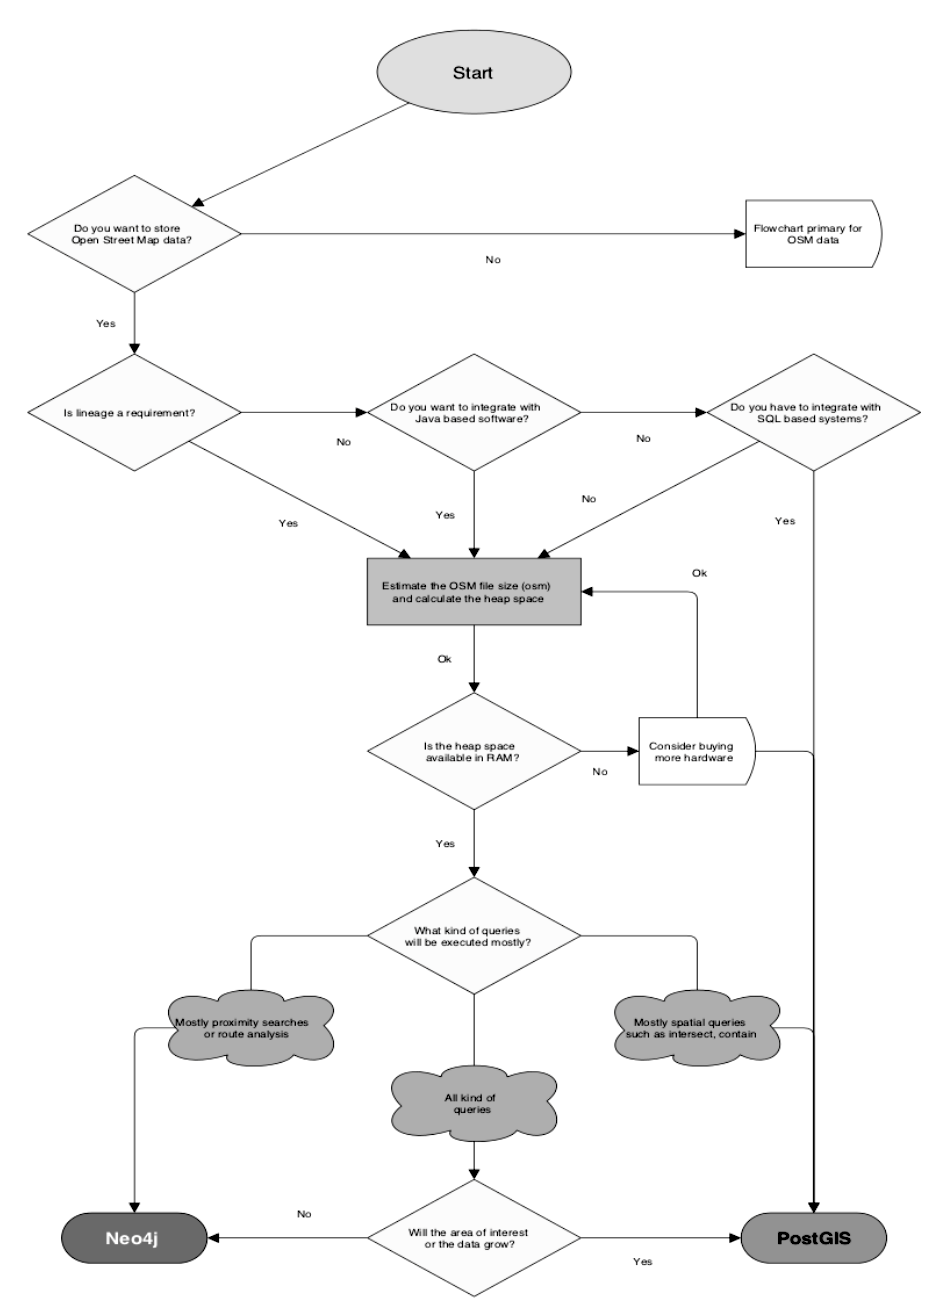
\includegraphics[width=\textwidth]{NeoVsPostgis}
    }%
    }%
    \caption{Neo4j Spatial vs PostGIS \cite{baas2012nosql}}
    \label{fig:NeoVsPostGIS}
\end{figure}